%% Copernicus Publications Manuscript Preparation Template for LaTeX Submissions
%% ---------------------------------
%% This template should be used for copernicus.cls
%% The class file and some style files are bundled in the Copernicus Latex Package, which can be downloaded from the different journal webpages.
%% For further assistance please contact Copernicus Publications at: production@copernicus.org
%% https://publications.copernicus.org/for_authors/manuscript_preparation.html

%% copernicus_rticles_template (flag for rticles template detection - do not remove!)

%% Please use the following documentclass and journal abbreviations for discussion papers and final revised papers.

%% 2-column papers and discussion papers
\documentclass[gc, manuscript]{copernicus}



%% Journal abbreviations (please use the same for discussion papers and final revised papers)


% Advances in Geosciences (adgeo)
% Advances in Radio Science (ars)
% Advances in Science and Research (asr)
% Advances in Statistical Climatology, Meteorology and Oceanography (ascmo)
% Annales Geophysicae (angeo)
% Archives Animal Breeding (aab)
% ASTRA Proceedings (ap)
% Atmospheric Chemistry and Physics (acp)
% Atmospheric Measurement Techniques (amt)
% Biogeosciences (bg)
% Climate of the Past (cp)
% DEUQUA Special Publications (deuquasp)
% Drinking Water Engineering and Science (dwes)
% Earth Surface Dynamics (esurf)
% Earth System Dynamics (esd)
% Earth System Science Data (essd)
% E&G Quaternary Science Journal (egqsj)
% Fossil Record (fr)
% Geochronology (gchron)
% Geographica Helvetica (gh)
% Geoscience Communication (gc)
% Geoscientific Instrumentation, Methods and Data Systems (gi)
% Geoscientific Model Development (gmd)
% History of Geo- and Space Sciences (hgss)
% Hydrology and Earth System Sciences (hess)
% Journal of Micropalaeontology (jm)
% Journal of Sensors and Sensor Systems (jsss)
% Mechanical Sciences (ms)
% Natural Hazards and Earth System Sciences (nhess)
% Nonlinear Processes in Geophysics (npg)
% Ocean Science (os)
% Primate Biology (pb)
% Proceedings of the International Association of Hydrological Sciences (piahs)
% Scientific Drilling (sd)
% SOIL (soil)
% Solid Earth (se)
% The Cryosphere (tc)
% Web Ecology (we)
% Wind Energy Science (wes)


%% \usepackage commands included in the copernicus.cls:
%\usepackage[german, english]{babel}
%\usepackage{tabularx}
%\usepackage{cancel}
%\usepackage{multirow}
%\usepackage{supertabular}
%\usepackage{algorithmic}
%\usepackage{algorithm}
%\usepackage{amsthm}
%\usepackage{float}
%\usepackage{subfig}
%\usepackage{rotating}


% The "Technical instructions for LaTex" by Copernicus require _not_ to insert any additional packages.
%
\usepackage{algorithmic}
\usepackage{algorithm}


\begin{document}

\title{GeoChronR -- an R framework to model and analyze age-uncertain paleogeoscientific timeseries.}


\Author[1]{Nicholas}{McKay}
\Author[2]{Julien}{Emile-Geay}
\Author[2]{Deborah}{Khider}


\affil[1]{School of Earth and Sustainability, Northern Arizona University, Flagstaff, AZ 86011}
\affil[2]{University of Southern California, Los Angeles, CA}

%% The [] brackets identify the author with the corresponding affiliation. 1, 2, 3, etc. should be inserted.



\runningtitle{The GeoChronR framework}

\runningauthor{McKay et al.}


\correspondence{Nicholas\ McKay\ (Nicholas.McKay@nau.edu)}



\received{}
\pubdiscuss{} %% only important for two-stage journals
\revised{}
\accepted{}
\published{}

%% These dates will be inserted by Copernicus Publications during the typesetting process.


\firstpage{1}

\maketitle


\begin{abstract}
Chronological uncertainty is a hallmark of the paleosciences. While many tools have been made available to researchers to produce age models suitable for various settings and assumptions, disparate tools and output formats often discourage integrative approaches. In addition, associated tasks like propagating age model uncertainties to subsequent analyses, and visualizing the results, have received comparatively little attention in the literature and available software. Here we describe GeoChronR, an open-source R package to facilitate these tasks. GeoChronR is built around emerging data standards for the paleosciences (Linked Paleo Data, or LiPD), and offers access to four popular age modeling techniques (Bacon, BChron, Oxcal, BAM). The output of these models is easily stored in LiPD, enabling paleo-aware synchronization, regression, correlation, principal component, and spectral analyses. Five real-world use cases illustrate how to use GeoChronR to facilitate these tasks, and to visualize the results in intuitive ways.
\end{abstract}


\copyrightstatement{The author's copyright for this publication is transferred to institution/company.}


\introduction

\subsection{Background}

Quantifying chronological uncertainties, and how they might influence the understanding of past changes is fundamental to the paleogeosciences.
Without robust error determination, it is impossible to properly assess the extent to which past changes occurred simultaneously across regions or the duration of abrupt events, both of which limit our capacity to apply paleoscientific understanding to modern and future processes.
The need for better infrastructure to both characterize uncertainty, and to explicitly evaluate how age uncertainty impacts the the interpretation of records of past climate, ecology or landscapes, has been long recognized \citep[(more)]{Noren2013}.
In response to this need, the paleogeoscience community has made substantial advances toward improving geochronological accuracy by:

\begin{enumerate}
\def\labelenumi{\arabic{enumi}.}
\item
  Improving analytical techniques that allow for more precise age determination on smaller and context-specific samples \citep[\citet{Eglinton96},\citet{Fifield2000},\citet{Eggins2005},\citet{Santos_blank_2010}]{Brown_radiocarbon89}
\item
  Refining our understanding of how past changes in the Earth system impact the age accuracy, for example: improvements to the radiocarbon calibration curve \citep[\citet{Stuiver98},intcal references]{Stuiver91} and advances in our understanding of spatial variability in cosmogenic production rates used in exposure dating \citep[\citet{Masarik2009}]{Balco2009}
\item
  Dramatic improvement in the level of sophistication and realism in age-depth models used to estimate the ages of sequences between dated samples \citep[e.g.][\citet{parnell2008flexible}, \citet{Blaauw2010CLAM}, \citet{Blaauw2011BACON}]{Ramsey2009Bayesian}.
\end{enumerate}

Over the past 20 years, these advances have been widely adopted in the paleogeosciences.
However, despite the progress made in quantifying uncertainty in ages and in age models, few studies have formally evaluated how chronological uncertainty may have affected their results.
For instance, whereas the algorithms presented by \citep[\citet{parnell2008flexible}, \citet{Blaauw2010CLAM}, \citet{Blaauw2011BACON}]{Ramsey2009Bayesian} have been broadly used, the overwhelming majority of these studies calculate the single best-estimate model (often a median or mean), use this model to put measured paleoclimatic or paleoenvironmental data on a timescale, and then proceed to analyze the record with little to no reference to the age modeling exercise \citep[\citet{McKay2009}]{McKay2008}.
Typically, any discussions of chronological uncertainties remain qualitative.

This paradigm is beginning to change.
In recent years a handful of studies have taken advantage of approaches that generate ensembles of age models to evaluate how the results of their analyses and conclusions vary given differences between ensemble members \citep[\citet{Rhines_JGR2011},\citet{Anchukaitis_Tierney2012},\citet{Shakun_Nature2012},\citet{Marcott_Science2013}, \citet{Tierney2013}]{Haam_Huybers2010}.
By using each ensemble age model to create a time-uncertain ensemble records, and then carrying that ensemble through the analysis, the precise impact of age uncertainty can be formally evaluated.
This approach, of course, does not address all aspects of uncertainty, but it does offer the broad potential to ascertain which results are robust to chronological uncertainty, and which are not.

Despite its potential to substantially improve uncertainty quantification for the paleogeosciences, this framework is not widely utilized.
The majority of studies utilizing this approach have been regional {[}e.g., \citet{Anchukaitis_Tierney2012},\citet{Tierney2013},\citet{mckay_onset_2018}, \citet{routson2018}\} or global-scale \citep[e.g.,][\citet{Marcott_Science2013},\citet{kaufman2020HoloceneGMST}]{Shakun_Nature2012} syntheses.
Occasionally, primary publications of new records incorporate time-uncertain analysis into their studies \citep[more]{Boldt2015}, but this remains rare.
We suggest that there are several reasons for the lack of adoption of these techniques:

\begin{enumerate}
\def\labelenumi{\arabic{enumi}.}
\item
  For synthesis studies, the necessary geochronological data are not publicly available for the vast majority of records. Even when they are available, the data are archived in diverse and unstructured data formats. Together, this makes what should be a simple process of aggregating and preparing data for analysis prohibitively time-consuming;
\item
  For studies of new and individual records, few tools for ensemble analysis are available, and those that are require a degree of comfort with coding languages and scientific programming that is rare among paleogeoscientists;
\item
  There is a disconnect between age-model development and time-uncertain analysis. Published approaches have utilized either simplified age-modeling approaches \citep{Haam_Huybers2010}, or specialized approaches not used elsewhere in the community \citep[\citet{Anchukaitis_Tierney2012},\citet{Marcott_Science2013},\citet{Tierney2013},\citet{routson2018}]{Shakun_Nature2012}.
\end{enumerate}

Extracting the relevant data from commonly-used age-modelling algorithms, creating time-uncertain ensembles, then reformatting those data for analysis in available tools typically requires the development of extensive custom codes. An integrative approach is needed to facilitate this work.

\subsection{Motivation}

GeoChronR was built to lower the barriers to broader adoption of these emerging methods.
It provides an easily-accessibly, open-source and extensible software package of industry-standard and cutting-edge tools that provides users with a single environment to create, analyse, and visualize time-uncertain data.
GeoChronR is designed around emerging standards in the paleogeosciences that connects users to growing libraries of standardized datasets formatted in the Linked PaleoData format \citep{LiPD} and \citep{neotoma}.

\subsection{Outline of manuscript}

This manuscript describes the design, analytical underpinnings and most common use cases of GeoChronR.
Section \ref{sec:age-modeling} describes the integration of age modelling algorithms with GeoChronR.
Section \ref{sec:age-uncertain-analysis} details the methods implemented for age uncertain analysis.
Section \ref{sec:visualization} goes through the principles and implementation of age-uncertain data visualization in GeoChronR, and section \ref{sec:use-cases} provides five real-world examples of how GeoChronR can be used for paleoscientific workflows.

\hypertarget{sec:age-modeling}{%
\section{Age Uncertainty Quantification in GeoChronR}\label{sec:age-modeling}}

GeoChronR does not introduce any new approaches to age uncertainty quantification; rather, it integrates existing, widely-used packages while streamlining the acquisition of age ensemble members.
Fundamentally, there are two types of age models used in the paleogeosciences: tie-point and layer-counted.
Most of the effort in age uncertainty quantification in the community has been focused on tie-point modelling, where the goal is to estimate ages (and their uncertainties) along a depth profile given chronological estimates (and their uncertainties) at multiple depths downcore.
Over the past 20 years, these algorithms have progressed from linear or polynomial regressions with simple characterizations of uncertainty \citep[\citet{heegaard05}]{clam} to more rigorous techniques, particularly Bayesian approaches: as of writing, the three most widely used algorithms are Bacon \citep{bacon}, BChron \citep{parnell2008flexible}, and OxCal \citep{ramsey2008deposition}, which are all Bayesian age-deposition models that estimate posterior distributions on age-depth relationships using different assumptions and methodologies.
\citet{trachsel2017} reviewed the performance of these three algorithms, as well as a non-Bayesian approach \citep{clam}, and found that the three Bayesian approaches generally outperform previous algorithms, especially when appropriate parameters are chosen (although choosing appropriate parameters can be challenging).
Bacon, BChron and Oxcal all leverage Monte Carlo Markov Chain (MCMC) techniques to sample the posterior distributions, thereby quantifiying age uncertainties as a function of depth in the section.
GeoChronR interfaces with each of these algorithms through their R packages \citep[\citet{oxcAAR}]{baconPackage} (cite other R Packages), streamlining input and output. \%data input and the extraction of the age ensembles from the MCMC results for further analysis.

In addition to working with ensembles from tie-point age models, GeoChronR connects users to probabilistic models of layer-counted chronologies. BAM \citep{BAM} was designed to probabilistically simulate counting uncertainty in banded archives, such as corals, ice cores, or varved sediments, but can be used to crudely simulate age uncertainty for any record, and is useful when the data or metadata required to calculate an age-depth model are unavailable. Here we briefly describe the theoretical basis and applications of each of the four approaches integrated in GeoChronR.

\subsection{Bacon}

The Bayesian ACcumulatiON (Bacon) algorithm \citep{bacon} is one of the most broadly used age-modelling techniques, and was designed to take advantage of prior knowledge about the distribution and autocorrelation structure of sedimentation rates in a sequence to better quantify uncertainty between dated levels.
The algorithm employs an adaptive Markov Chain Monte Carlo algorithm that allows for Bayesian learning to update the sedimentation rate distribution.
Bacon has two key parameters: the shape of the accumulation prior, and the segment length, which can interact in complicaed ways \citep{trachsel2017}.
In our experience, the segment length parameter has the greatest impact on the ultimate shape and amount of uncertainty simulated by Bacon, as larger segments result in increased flexibility of the age-depth curve, and increased uncertainty between dated levels.
Bacon is written in C++ and R, with an R interface.
More recently, the authors released an R package \texttt{rbacon} \citep{baconPackage}, which GeoChronR leverages to provide access to the algorithm.
Bacon will optionally return a subset of the MCMC accumulation rate ensemble members with high \emph{a posteriori} probabilities, which GeoChronR uses to form age ensemble members for subsequent analysis.

depositional model?

\subsection{BChron}

BChron \citep[\citet{parnell2008flexible}]{bchron} uses a similar approach, using a continuous Markov monotone stochastic process coupled to a piecewise linear deposition model. This simplicity allows semi-analytical solutions that make BChron computationally efficient. BChron was originally intended to model radiocarbon-based age-depth models in lake sedimentary cores of primarily Holocene age, but its design allows broader applications. In particular, modeling accumulation as additive independent gamma increments is appealing for the representation of hiatuses, particulary for speleothem records, where accumulation rate can vary quite abruptly between quiescient intervals of near-constant accumulation \citep[\citet{PRYSM},\citet{Hu_epsl17}]{Parnell_QSR2011}. The downside of this assumption is that BChron is known to exaggerate age uncertainties in cases where sedimentation varies smoothly \citep{trachsel2017}.

Adjustable parameters? \{Deborah\}

\subsection{Oxcal}

The OxCal software package has a long history and extensive tools for the statistical treatment of radiocarbon and other geochronological data \citep{BronkRamsey95}.
In \citet{ramsey2008deposition}, age-depth modelling was introduced with three options for modelling depositional processes that are typically useful for sedimentary sequences: uniform, varve, and Poisson deposition models, labeled U-sequence, V-sequence and P-sequence, respectively.
The Poisson-based model is the most broadly applicable for sedimentary, or other accumulation-based archives (e.g.~speleothems), and although any sequence type can be used in GeoChronR, most users will use a P-sequence, which is the default.
Analagously to segment length parameter in Bacon, the \emph{k} parameter (called ``eventsPerUnitLength'' in GeoChronR), controls how many events are simulated per unit of depth, and has a strong impact on the flexibility of the model, as well as the amplitude of the resulting uncertainty.
As the number of events increases, the flexibility of the model, and the uncertainties decrease.
\citet{trachsel2017} found that this parameter has large impact on the accuracy of the model, and moreso than the choices made in Bacon or Bchron.
Fortunately, \citet{bronkramsey2010} made it possible for \emph{k} to be treated as a variable, and the model will estimate the most likely values of \emph{k} given a prior estimate and the data, however this calculation can greatly increase the convergence time of the model.
Oxcal is written in C++, with an interface in R \citep{oxcAAR}.
Oxcal doesn't calculate posterior ensembles for a depth sequence, but can optionally output MCMC posteriors at specified levels in the sequence.
GeoChronR uses this feature to extract ensemble members for subsequent analysis.

\subsection{Banded Age Model (BAM)}

\citet{BAM} is a probabilistic model of age errors in layer-counted chronologies. The model allows a flexible parametric representation of such errors (either as Poisson or Bernoulli processes), and separately considers the possibility of double-counting or missing a band. The model is parameterized in terms of the error rates associated with each event, which are intuitive parameters to paleogeoscientists, and may be estimated via replication \citep{DeLong_Paleo3_2013}. In cases where such rates can be estimated from the data alone, an optimization principle may be used to identify a more likely age model when a high-frequency common signal can be used as a clock \citep{BAM}. As of now, BAM does not consider uncertainties about such parameters, representing a weakness of the method. Bayesian generalizations have been proposed \citep{BoersCP2017}, which could one day be incorporated into GeoChronR if the code is made public.

BAM was coded in MATLAB and R, and it is this latter version that GeoChronR uses.

\hypertarget{sec:age-uncertain-analysis}{%
\section{Age-uncertain data analysis in GeoChronR}\label{sec:age-uncertain-analysis}}

Some theoretical work has attempted to quantify how chronological uncertainty may affect various paleoscientific inferences \citep[e.g.][]{HuybersWunsch2004}; however, such an approach is necessarily piecemeal, and therefore impractical given the variety of age-uncertainty structures in real-world paleogeoscientific data.
Consequently, GeoChronR follows a pragmatic and broadly-used approach that leverages age ensembles, and optionally ensembles in climate proxy or paleoenvironmental data, to propagate uncertainties through all steps of an analysis.
Effectively, this is done by randomly sampling from the ensemble(s) and then repeating the analysis on each sample (typically hundreds to thousands) to build an output ensemble that quantifies the impact of those uncertainties on a particular inference.
These output ensembles often do not lend themselves to binary significance statistics (e.g., a p-value below), but are readily used to provide quantiles that estimate probability density ranges, and can provide strong evidence for which results are robust to age and proxy uncertainty (and which are not).
Version 1.0.0 of GeoChronR has implemented ensemble analytical techniques for four of the most common analyses in the paleogeosciences: correlation, regression, spectral and principal component analyses.

\subsection{Correlation}

Pearson's product-moment correlation is the most common measure of association between variables.\\
Its computation is fast, lending itself to ensemble analysis, with a handful of pretreatment and significance considerations that are relevant for ensembles of paleogeoscientific data.

First, correlation analysis for timeseries is built on the assumption the datasets can be aligned on a common timeline. Age-uncertain data violate this assumption.
We overcome this by treating each ensemble member from one or more age uncertain timeseries as valid for that iteration, then ``bin'' each of the timeseries into coeval intervals.
The ``binning'' procedure in GeoChronR sets up an interval, which is typical evenly spaced, over which the data are averaged.
Generally, this intentionally degrades the median resolution of the timeseries, for example, a timeseries with 37-year median spacing could be reasonably ``binned'' into 100- or 200-year bins.
The binning procedure is repeated for each ensemble member, meaning that between different ensembles, different observations will be placed in different bins.

Following binning, Pearson correlation is calculated and recorded for each ensemble member.
In addition to the correlation coefficients, GeoChronR calculates their significance for each correlation.
Paleogeoscientific timeseries are often highly autocorrelated, which can lead to spurious assessments of significance \citep{Hu_epsl17}.
Therefore, in addition to the standard Student's T-test p-value calculation, we also calculate a p-value that is adjusted for autocorrelation to reflect the reduction in degrees of freedom due to autocorrelation following \citet{bretherton1999}. However, repeating this test over multiple ensembles raises the issue of test multiplicity \citep{Ventura2004}, or ``look elsewhere effect''. To overcome this problem, we control for this false discovery rate using the simple approach of \citet{BenjaminiHochberg95}, coded in R by \citet{Ventura2004}.

\subsection{Regression}

Linear regression is a commonly used tool to model the relationships between paleogeoscientific data and instrumental or other datasets.
One application is calibration-in-time {[}references{]}, whereby a proxy timeseries is calibrated to an instrumental series with a linear regression model over their period of overlap.
This approach is particularly vulnerable to age uncertainties, as both the development of the relationship, and the reconstruction, are affected.
GeoChronR propagates age (and optionally proxy) uncertainties through both the fitting of the ordinary least squares regression model, and the reconstruction ``forecast'' using the ensemble model results and age uncertainty.
Like the correlation algorithm, ensemble regression uses an ensemble binning procedure that's analgous to correlation.
GeoChronR then exports uncertainty structure of the modeled parameters (e.g.~slope and intercept), as well as the ensemble of reconstructed calibrated data through time.

\subsection{Principal Component Analysis}

GeoChronR implements the age-uncertain principal component analysis (PCA) procedure introduced by \citet{anchukaitis2013mceof}, with some minor modifications and additions.
Like correlation and regression, PCA (or empirical orthogonal function \{EOF\} analysis) requires temporally aligned observations, and GeoChronR uses a binning procedure to achieve this across multiple ensembles.
This differs from the implementation of \citet{anchukaitis2013mceof}, who interpolated the data to a common timestep.
In addition, traditional singular value decomposition approaches to PCA require a complete set of observations without any missing values.
For paleoclimate data, especially when considering age uncertainty, this requirement is often prohibitive.
To overcome this, GeoChronR implements multiple options for PCA analysis using the \texttt{pcaMethods} package.
The default and most rigorously tested option is a probabilistic PCA (PPCA) approach that uses expectation maximization algorithms to infill missing values \citep{roweis1998algorithms}.
This algorithm assumes that the data and their uncertainties are normally distributed, which is often (but not always) a reasonable assumption for paleogeoscientific data.
As in correlation and regression, GeoChronR propagates uncertainties through the analysis by repeating the analysis across randomly sampled age and/or proxy ensemble members to build output ensembles of the loadings (eigenvectors), variance explained (eigenvalues) and principal component timeseries.
Because the sign of the loadings in PCA analyses is arbitrary and vulnerable to small changes in the input data, GeoChronR reorients the sign of the loadings for all PCs so that the mean of the loadings is positive.
For well defined modes this effectively orients ensemble PCs, but loading orientation may be uncertain for lower order, or more uncertain, modes.

\hypertarget{sec:spec_theory}{%
\subsection{Spectral Analysis}\label{sec:spec_theory}}

Many research questions in the paleosciences revolve around spectral analysis: describing phase leads and lags among different climate system components over the Pleistocene \citep[SPECMAP,][]{imbrie1984orbital}, the hunt for astronomical cycles over the Holocene \citep[\citet{bond2001}]{mill_monograph} or in deep time \citep[\citet{Meyers_2012},\citet{Meyers_2015}]{MeyersSageman_2007}, or characterizing the continuum of climate variability \citep[\citet{ZhuPNAS2019}]{Huybers_Curry2006}. Yet, spectral analysis in the paleosciences faces unique challenges: chronological uncertainties, of course, as well as uneven sampling, which violates the assumptions of classical spectral methods \citep{Ghil02}.

To facilitate the quantification of chronological uncertainties in such assessments, GeoChronR implements 4 spectral approaches:
1. the Lomb-Scargle periodogram \citep{VanderPlas_2018}, which uses an inverse approach to harmonic analysis in unevenly-spaced timeseries.\\
2. REDFIT, a version of the Lomb-Scargle periodogram tailored to paleoclimatic data \citep[\citet{Mudelsee_02}, \citet{Mudelsee_NPG09}]{SchulzMudelsee_02}. The R implementation of REDFIT is inhereted from the dplR package \citep{Bunn2008115}.
3. the wavelet-based method of \citet{Mathias_JSS04}, called \texttt{nuspectral}. This method is quite similar to the Weighted Wavelet Z-transform algorithm of \citet{Foster_AJ96}, though it is prohibitively slow in this implementation, and the fast version using a compact-support approximations of the mother wavelet did not perform well in our tests.
4. The multi-taper method (MTM) of \citet{thomson82}, a mainstay of spectral analysis \citep{Ghil02} designed for evenly spaced timseries. GeoChronR re-uses its \citet{astrochron} implementation, which couples MTM to efficient linear interpolation, together with various utilities to define autoregressive and power-law benchmarks for spectral peaks.

\hypertarget{sec:visualization}{%
\section{Visualization with GeoChronR}\label{sec:visualization}}

One of the challenges with age-uncertain analysis is that it adds at least one additional dimension to the results, which can be challenging to visualize.
GeoChronR aims to facilitate simple creation of intuitive, publication-quality figures that provide multiple options for visualizing the impacts of age-uncertainty, while maintaining flexibility for users to customize their results as needed.
To meet the multiple constraints of simplicity, quality and customization, GeoChronR relies heavily on the \texttt{ggplot2} package \citep{ggplot2}.
High-level plotting functions in GeoChronR (e.g., \texttt{plotTimeseriesEnsRibbons} and \texttt{plotPca}) produce complete figures as \texttt{ggplot2} objects, that can be readily customized by adding or changing \texttt{ggplot2} layers.
The figures in the Use Cases section (Section @(sec:use-cases)) are all produced directly from GeoChronR without modification and generally fall into a few categories.

\{Light Mode vs Dark Mode\}

\subsection{Timeseries}

Most of the figures that GeoChronR produces are ensemble timeseries.
GeoChronR uses two complementary approaches to visualize these ensembles.
The first is the simplest, where a large subset of the ensemble members are plotted as semi-transparent lines.
This approach, implemented in \texttt{plotTimeseriesEnsLines}, provides a faithful representation of the data, while the overlapping semi transparency provides a qualitative sense of the ensemble uncertainty structure.
The second approach uses contours to more rigorlously visualize the structure of the time-value uncertainty space represented by the ensembles.
\texttt{plotTimeseriesEnsRibbons} shows the quantiles of the ensembles at specified levels as shaded bands.
This approach provides the quantitative uncertainty structure, but tends to smooth out the apparent temporal evolution of the data.
Fortunately, the two approaches are complementary, and often the best approach is to quantify the ensemble distribution with ribbons in the background, and then overlap them with a handful of ensemble lines to illustrate the structure in representive ensemble members.

\subsection{Maps}

GeoChronR has simple mapping capabilities built in that rely on the \texttt{maps} \citep{maps} and \texttt{ggmap} \citep{ggmap} packages.
The \texttt{mapLipd} and \texttt{mapTs} functions provide quick geospatial visualization of one or more datasets, but also serve as the basis for the visualization of ensemble spatial data produced by ensemble PCA analyses.
In paleogeoscientific studies, the loadings (eigenvectors) of a PCA analysis are often portrayed as dots on a map, with a colorscale that highlights the sign and amplitude of the loadings.
In ensemble PCA, the additional dimension of uncertainty in the loadings needs to be visualized as well.
In GeoChronR, the median of the loadings is shown as a color, and the size of the symbol is inversely proportional to the spread of uncertainty across the ensemble.
Consequently, large symbols depict loadings that are robust to the uncertainties, whereas small symbols show datasets whose loadings change substantially across the analysis.
An example is shown in Section @(sec:pca)

\subsection{Spectra}

It is customary to plot spectra on a log-log scale, which helps separate close-by frequencies. This choice also naturally highlights scaling laws \citep[\citet{ZhuPNAS2019}]{lovejoy2013weather} as linear structures in this reference frame. GeoChronR thus implements this convention. In addition, the abscissa (\(\log_{10} f\)) is labeled according to the corresponding period, which are more intuitive than frequency to scientists reading the plot. To help identify significant periodicities, confidence limits can be superimposed, based on user-specified benchmarks (see \ref{sec:use-cases}). The \texttt{plotSpectrum()} function visualizes single ensemble members (e.g.~a median age model), while \texttt{plotSpectraEns()} visualizes the quantiles of a distribution of age-uncertain spectra as ribbons, using the eponymous \texttt{ggplot} function.

\hypertarget{sec:use-cases}{%
\section{Use cases}\label{sec:use-cases}}

We now illustrate the use of these tools on five use cases. The first example shows how to create age ensembles on different archives, and how to visualize the timing of abrupt events with appropriate uncertainty quantification. The second example shows how to quantify similarities in age-uncertain records. The third introduces the topic of age-uncertain calibrations, the fourth quantifies multivariate relationships using principal components analyses, and the fifth deal with spectral analysis.

\subsection{Creating an age ensemble}

A common first task when using geoChronR is to create an age ensemble, either because the user is developing a new record, or because the age ensemble data for the record they are interested is unavailable.
As described in section X.Y, workflows for four published age quantification programs are integrated into geoChronR.
All four methods are simply used in geoChronR with a LiPD file that contains the chronological measurements, and the functions \texttt{runBacon(L)}, \texttt{runBchron(L)}, \texttt{runOxcal(L)} and \texttt{runBam(L)}.
These functions take LiPD objects as inputs, and return updated LiPD objects that include age-ensemble data generated by the respective software packages, with these data stored in appropriate tables.
Typically, additional parameters are needed for to optimally run the algorithms.
When these parameters are not included, geoChronR will run in interactive mode, asking the user which variables and parameters they would like to model.
These parameter choices are printed to the screen during while the program runs, or are available later with the function \texttt{getLastVarString()}.
By specifying these parameters, age model creation can be scripted and will run in non-interactive mode.
In this use case, we'll use geoChronR and BChron \citep{parnell2008flexible} to calculate an age ensemble for the Hulu Cave \(\delta^{18}\)O speleothem record \citep{hulu2001}, and BAM \citep{BAM} to simulate age uncertainties for the GISP2 ice core \(\delta^{18}\)O dataset \citep{alley}.
The \texttt{plotChronEns(hulu)} function will plot an age-depth model and uncertainties derived from the age ensemble.

\begin{figure}
\centering
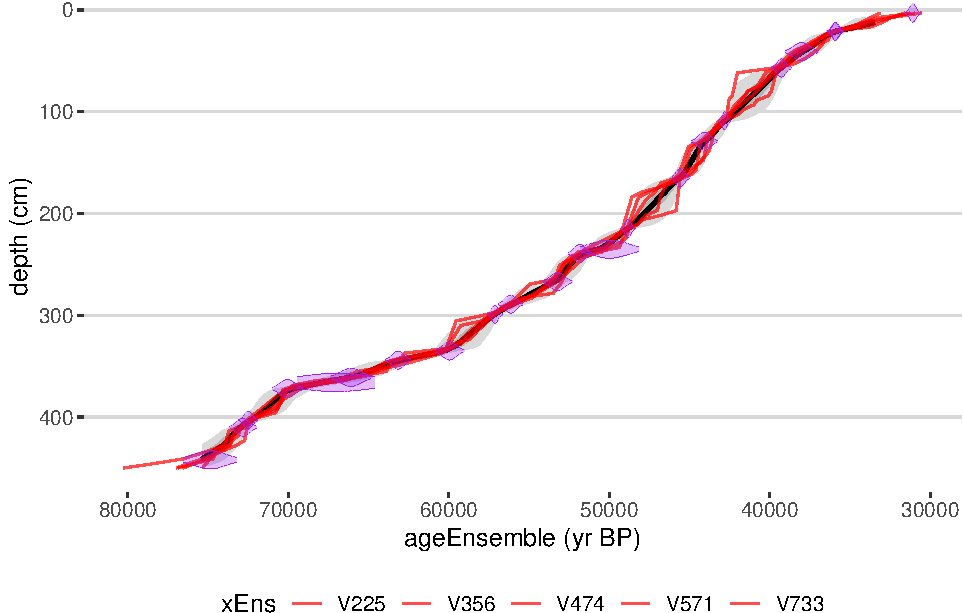
\includegraphics{geoChronR-paper_files/figure-latex/unnamed-chunk-4-1.pdf}
\caption{\label{fig:unnamed-chunk-4}Need to write a caption}
\end{figure}

After an age ensemble has been added to a LiPD object, the user can visualize the ensemble timeseries using \texttt{plotTimeseriesEnsRibbons()} and \texttt{plotTimeseriesEnsLines()}.
GISP2 \(\delta^{18}\)O is plotted with age uncertainty, using both functions, in figure x.

\begin{figure}
\centering
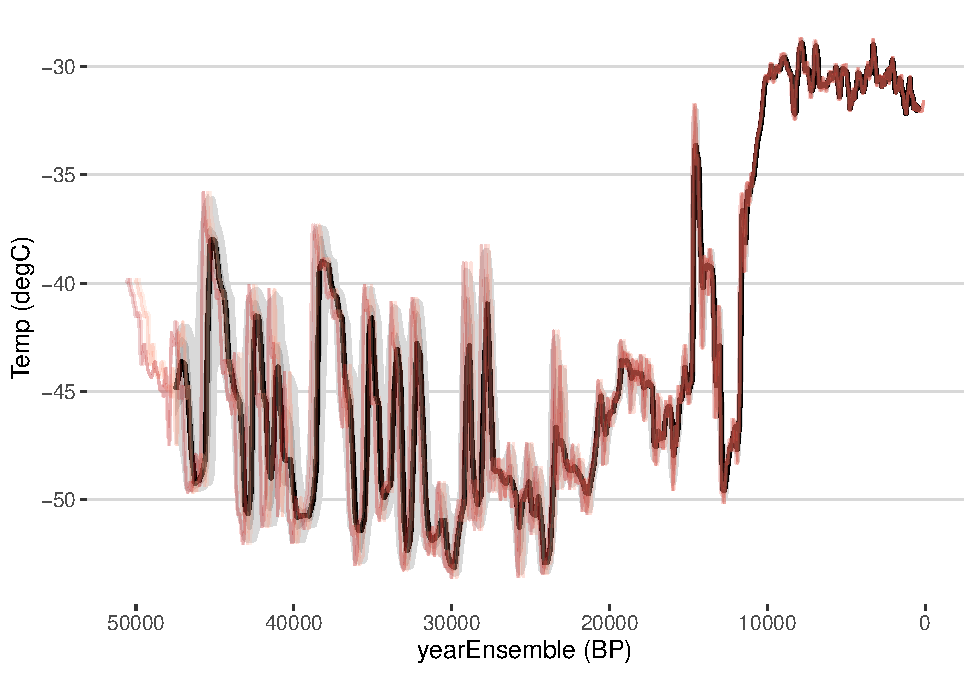
\includegraphics{geoChronR-paper_files/figure-latex/unnamed-chunk-6-1.pdf}
\caption{\label{fig:unnamed-chunk-6}Need to write a caption}
\end{figure}

\subsection{Correlation}

Now that the user has generated age ensembles for the two datasets, they're interested to see if a correlation between the two datasets is robust to the age uncertainty modeled here.
On multi-millennial timescales, the two datasets dislay similar features, and previous work has suggested that abrupt events of the Last Glacial period, which are observed in the GISP2 record, can impact the Asian Monsoon and be observed is speleothem records such as the Hulu Cave dataset. (NM: add references here and flesh out background)
The \texttt{corEns()} function in geoChronR will calculate ensemble correlations across age-uncertain datasets, such as these.
\texttt{corEns()} will also sample across ensembles in the paleoData as well, if present.
Here we calculate correlations during the period of overlap in 500 yr steps, determining significance for each pair of ensemble members while accounting for autocorrelation.

The results show consistently negative correlations, although 14.08\% of the ensemble members are positive.
However, only 0.89\% are significant after accounting for serial autocorrelation.

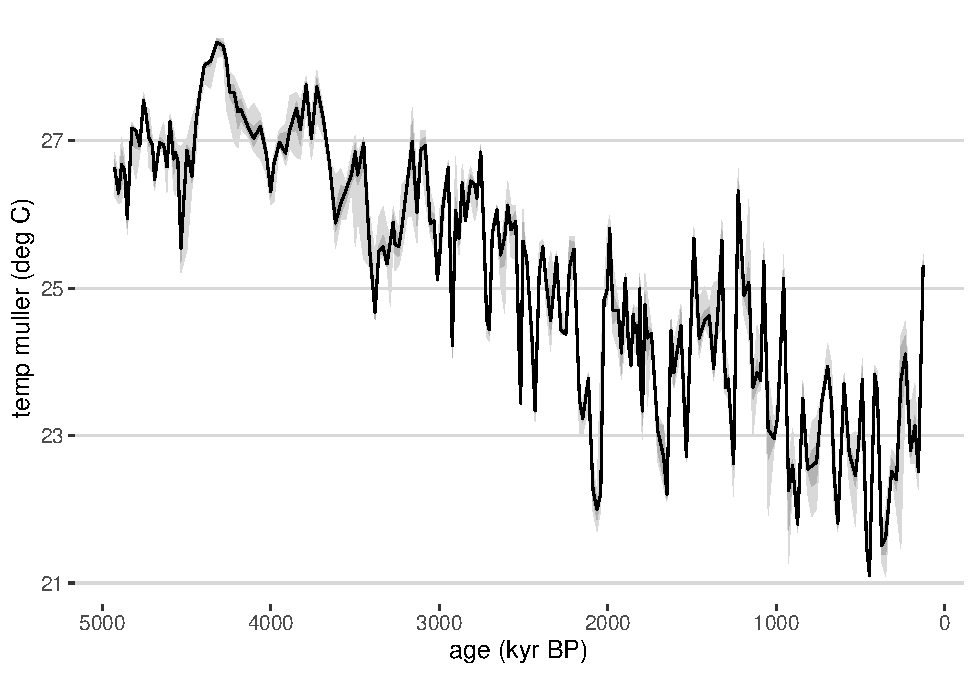
\includegraphics{geoChronR-paper_files/figure-latex/unnamed-chunk-8-1.pdf} 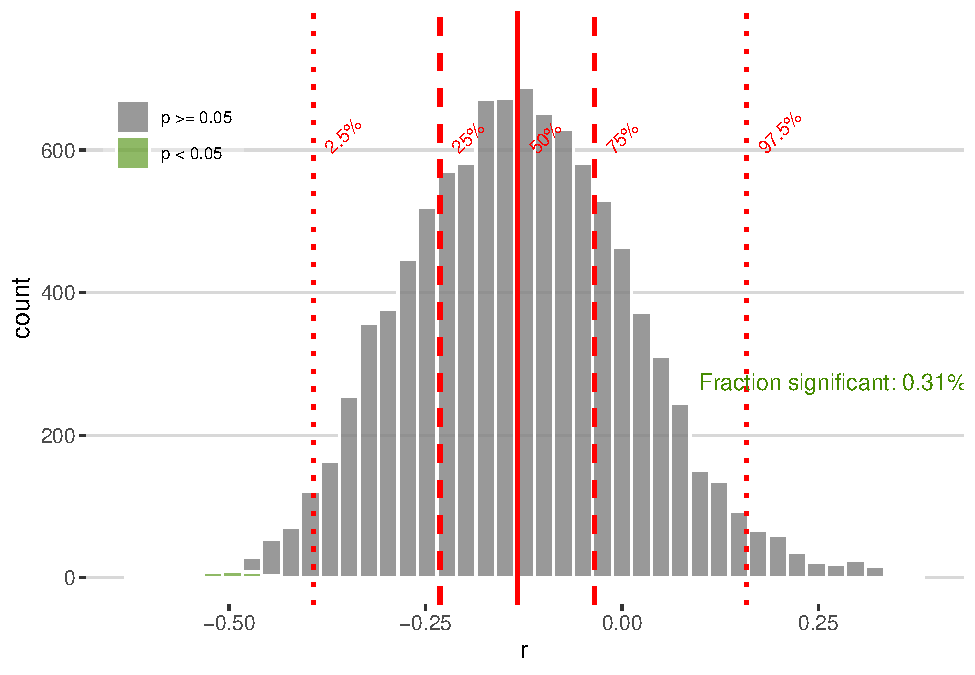
\includegraphics{geoChronR-paper_files/figure-latex/unnamed-chunk-8-2.pdf}

In this use case, we demonstrate how a user could calculate and visualize and age-uncertain correlation between the Hulu speleothem \(\delta^{18}\mathrm{O}\) record and the GISP2 ice core \(\delta^{18}\mathrm{O}\) record. (Introduction about why a user might want to do an age uncertain correlation between Hulu and GISP2).

\subsection{Age-uncertain Calibration}

A natural extension of ensemble correlation is ensemble regression.
Although there are use cases where regressing one age-uncertain variable onto another is called for, here we regress an age-uncertain paleoclimate proxy onto time-certain instrumental to develop a calibration-in-time.
For this use case, we reproduce the results of \citet{Boldt:2015}, where the authors calibrate a spectral reflectance measure of chlorophyll abundance to temperature in Northern Alaska.

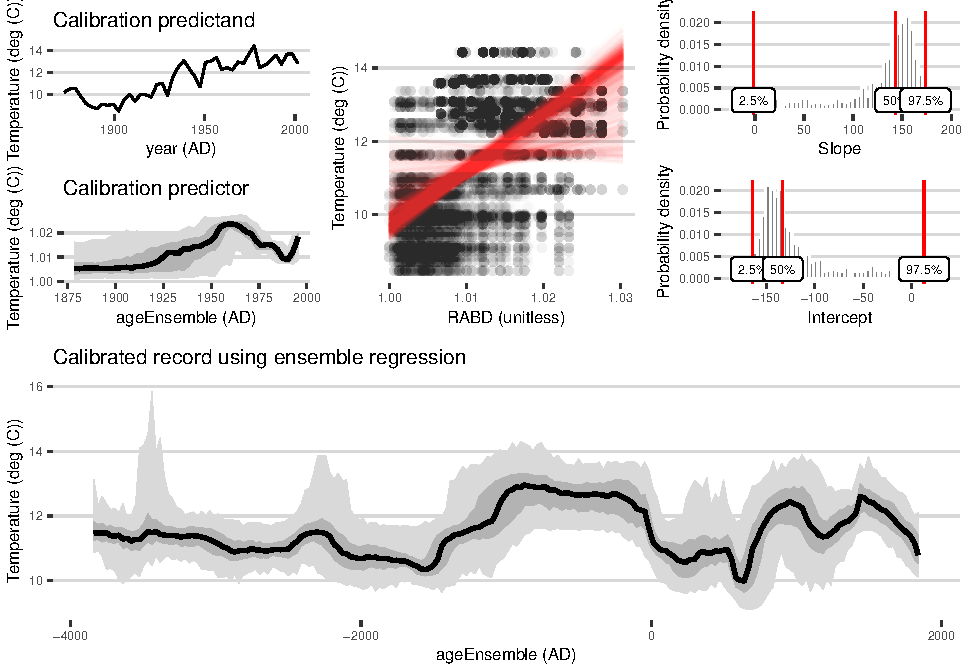
\includegraphics{geoChronR-paper_files/figure-latex/unnamed-chunk-10-1.pdf}
Figure captions.

\subsection{Principle Component Analysis \{sec:pca\}}

Thus far, the use cases have highlighted age-uncertain analyses of one or two sites, however quantifying the effects of age uncertainty can be even more impactful over large spatial datasets.
Here we showcase how to use geoChronR to perform age-uncertain principle components analysis (PCA), also known as Monte Carlo Empirical Orthogonal Function (MCEOF) analysis, pioneered by \citet{anchukaitis2013mceof}.
In this example, we examine the Arctic 2k database \citep{McKayKaufman2014}.

\begin{figure}
\centering
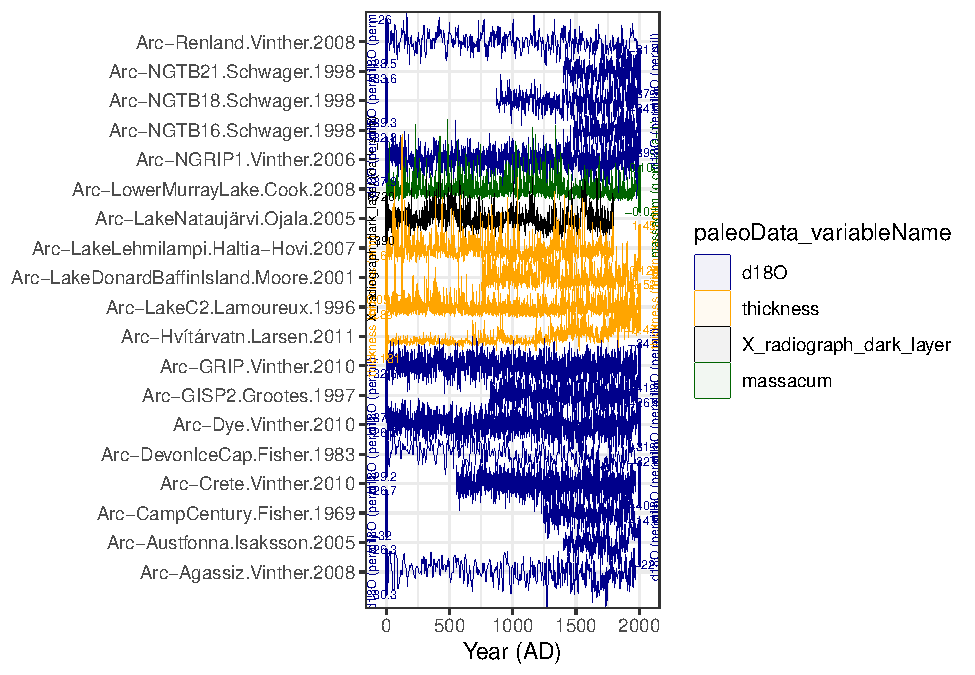
\includegraphics{geoChronR-paper_files/figure-latex/unnamed-chunk-12-1.pdf}
\caption{\label{fig:unnamed-chunk-12}Need to write a caption}
\end{figure}

\begin{figure}
\centering
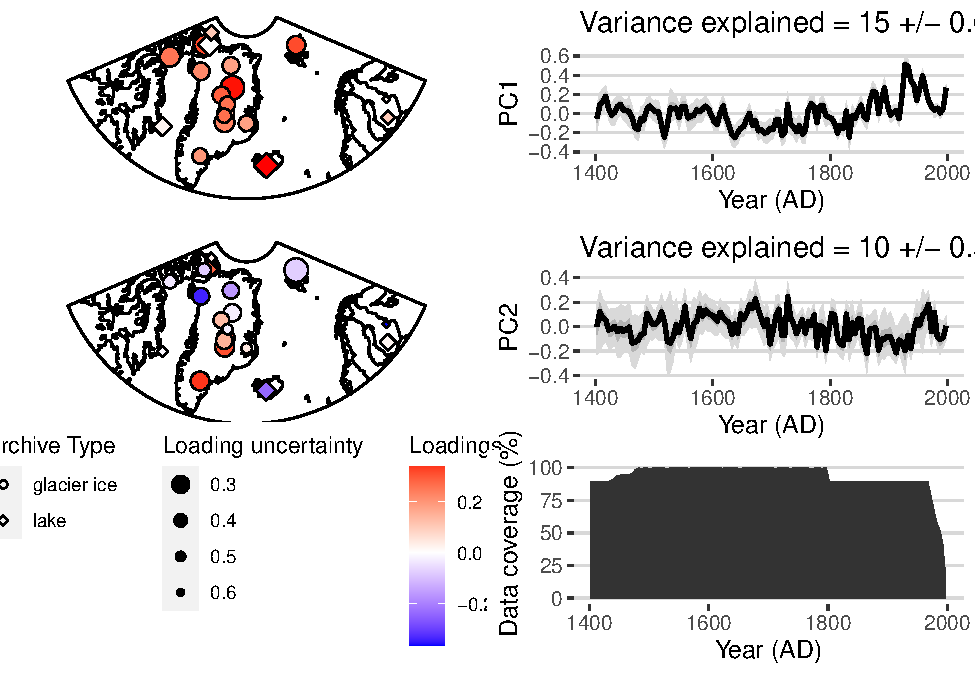
\includegraphics{geoChronR-paper_files/figure-latex/unnamed-chunk-14-1.pdf}
\caption{\label{fig:unnamed-chunk-14}Need to write a caption}
\end{figure}

\subsection{Spectral Analysis}

To illustrate the use of spectral analysis functionalities, consider the following use case: a paleoceanographer wants to identify the relative energy of oscillations at orbital (Milankovitch) periodicities in a deep-sea sediment core, and quantify the impact of age uncertainties on this assessment. To do so, they select the benthic \(\delta^{18}\mathrm{O}\) record of the International Ocean Drilling Project core 846 \citep[\citet{Shackleton95}]{mix1995benthic}, covering the past 4.7 million years. For this assessment, we use a new age model obtained by alignment to the benthic \(\delta^{18}\mathrm{O}\) stack of \citet{LisieckiRaymo05} using the HMM-Match algorithm \citep[\citet{Khider_2017}]{ProbStack}. HMM-Match is a probabilistic method that generates an ensemble of 1000 possible age models compatible with the chronostratigraphic constraints; this ensemble was archived as a table in the associated \href{http://lipdverse.org/geoChronR-examples/ODP846.Lawrence.2006.lpd}{LiPD file}.

Now let us take a first look at the median age model:

\begin{figure}
\centering
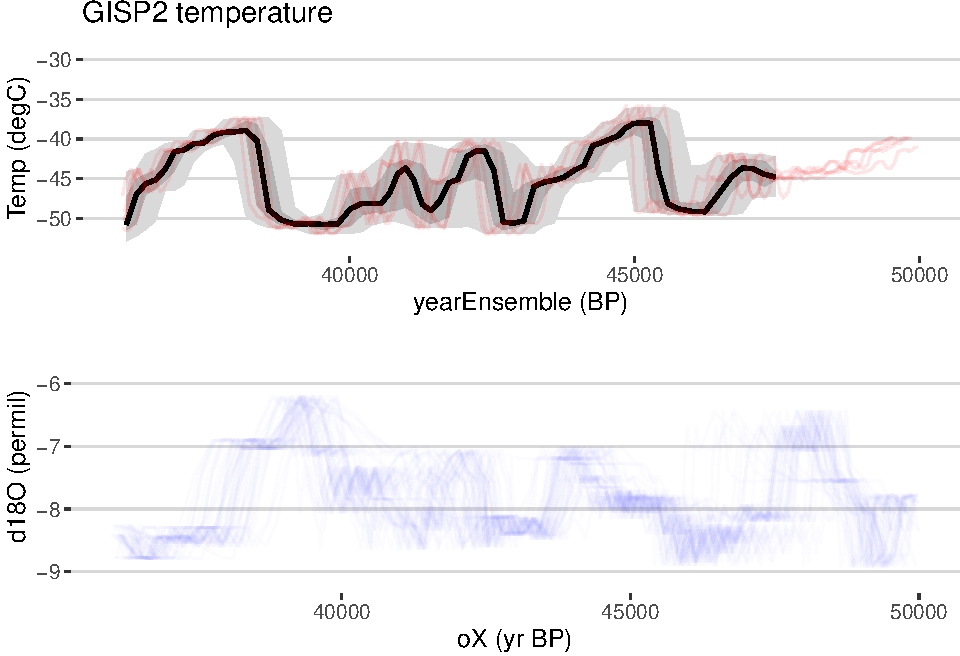
\includegraphics{geoChronR-paper_files/figure-latex/unnamed-chunk-16-1.pdf}
\caption{\label{fig:unnamed-chunk-16}Need to write a caption}
\end{figure}

This paleoclimate record displays three salient features:

\begin{itemize}
\item
  a long-term cooling trend characteristic of the late Neogene and Quaternary climate.
\item
  quasi-periodic oscillations (the legendary Pleistocene Ice Ages)
\item
  nonstationary behavior, related to the well-known mid-Pleistocene transition from a ``41k world'' to a ``100k world'' somewhere around 0.8 Ma \citep{Paillard_2001}.
\end{itemize}

For tractability, let us focus on the last million years, and use the median age model. As mentioned in @ref(sec:spec\_theory) a standard assumption of spectral analysis is that data are evenly spaced in time. In real-world paleo timeseries this is seldom the case. Indeed, over the past 1 Ma, the time increments (\(\Delta t\)) are sharply peaked around 2 ka, but they range from 0 to about 7.5 ka. For now, let us assume that the time axis, albeit uneven, is known without uncertainty. From this point there are two ways to proceed: 1) use methods that explictly deal with unevenly-spaced data, or 2) interpolate to a regular grid and apply standard methods (see @ref(sec:spec\_theory)). Though GeoChronR supports four different methods, we will highlight only two here: REDFIT and MTM.

\includegraphics{geoChronR-paper_files/figure-latex/REDFIT-1.pdf}

It is clearly seen that the data contain significant energy (peaks) near, but not exactly at, the famed Milankovitch periodicities (100, 41, 23, and 19 kyr). These periodicities (particularly the eccentricity (100kyr) and precessional (23 and 19 kyr)) rise above the null (the 95\% quantile from an autoregressive process of order one, see \citet{Mudelsee_NPG09}). The obliquity period is relatively weak, and does not rise above the AR(1) benchmark.

The Lomb-Scargle periodogram used by REDFIT is a decent way to deal with unevenly-spaced timeseries, but it is still a periodogram, which has several problems. In particular, it is inconsistent: the variance of each estimate goes to infinity as the number of observations increases. This is mitigated somewhat with the application of Welch's Overlapping Segment Averaging, but whose parameter choice is fairly arbitrary. On the other hand, MTM \citep{thomson82} is an optimal estimator, which is consistent (the more data, the better constrained the amplitude of the peaks). Formally, MTM optimizes the classic bias-variance tradeoff inherent to all statistical inference. It does so by minimizing speactral leakage outside of a frequency band with half-bandwidth equal to \(pf_R\), where \(f_R=1/(N \Delta t)\) is the Rayleigh frequency, \(\Delta t\) is the sampling interval, \(N\) the number of measurements, and \(p\) is the so-called \emph{time-bandwidth product} \citep{Ghil02}. \(p\) can only take a finite number of values, all multiples of 1/2 between 2 and 4. A larger \(p\) means lower variance (i.e.~less uncertainty about the power), but broader peaks (i.e.~a lower spectral resolution), synonymous with more uncerainty about the exact location of the harmonic. So while MTM might not distinguish between closely-spaced harmonics, it is much less likely to identify spurious peaks, especially at high frequencies. In addition, a battery of formal tests have been devised with MTM, allowing under reasonably broad assumptions to ascertain the significance of spectral peaks. We show how to use this ``harmonic F-test'' below.

The classic version of MTM can only handles evenly-spaced data. As we saw above, the data are not that far from evenly-spaced, so is is reasonable to interpolate them using standard methods. Conveniently, both the interpolation routine and MTM are available within the \citep[astrochron][]{astrochron} package, which is thus a dependency of GeoChronR.

\conclusions

Version 1.0.0 of GeoChronR provides user-friendly access to common age-uncertain analyses in the paleogeosciences, along with intuitive visualization of the results.
Although the focus has been on simplicity and ease of use, GeoChronR also has the underlying infrastructure to support customized analyses for users seeking to address a more nuanced or complex question.
Nevertheless, in many ways the paleogeoscience community is only scratching the surface with age-uncertain analysis, and we look forward to working with the community to extend and expand the package.
Looking forward, we suggest that the next major direction for age-uncertain analysis is philosophical, not technical.
Thus far, the community (and GeoChronR) has focused on quantifying the range of possibilities presented by age-uncertainty, not on developing approaches to constrain which ensemble members are most likely.
Theoretically, additional information from nearby records, forcings or covariance structures could do so, but little has been done to date \citep{wernerAndTingley}.

GeoChronR is open-source community-sofware, and has benefitted substantially from multiple contributors and input from early adopters and workshop participants. {[}should we list them here?{]}
We welcome feedback and strongly encourage contributions and enhancements, via the \href{https://github.com/nickmckay/GeoChronR/issues}{GitHub issue tracker}.

Subsection text here.

\subsubsection{Subsubsection Heading Here}

Subsubsection text here.

\section{Content section with citations}

See the \href{http://rmarkdown.rstudio.com/authoring_bibliographies_and_citations.html}{R Markdown docs for bibliographies and citations}.

Copernicus supports biblatex. I put the .bib entries from the Paleocube proposal into \texttt{geochronr.bib}. Citations work like this:

Read \citep{Evans_QSR13}, and \citep[see][]{PRYSM}.

\section{Content section with list}

If you want to insert a list, you must

\begin{itemize}
\item
  leave
\item
  empty lines
\item
  between each list item
\end{itemize}

\begin{verbatim}
- leave

- empty lines

- between each list item
\end{verbatim}

\section{Examples from the official template}

\subsection{FIGURES}

When figures and tables are placed at the end of the MS (article in one-column style), please add \clearpage between bibliography and first table and/or figure as well as between each table and/or figure.

\subsection{TABLES}

You can ad \LaTeX table in an R Markdown document to meet the template requirements.

\subsubsection{ONE-COLUMN TABLE}

\textbackslash{}begin\{table\}{[}t{]}

\caption{TEXT}

\textbackslash{}begin\{tabular\}\{l c r\}
\tophline

\subsection{PHYSICAL UNITS}

Please use \texttt{\textbackslash{}unit\{\}} (allows to save the math/\texttt{\$} environment) and apply the exponential notation, for example \(3.14\,\unit{km\,h^{-1}}\) (using LaTeX mode: \texttt{\textbackslash{}(\ 3.14\textbackslash{},\textbackslash{}unit\{...\}\ \textbackslash{})}) or \unit{0.872\,m\,s^{-1}} (using only \texttt{\textbackslash{}unit\{0.872\textbackslash{},m\textbackslash{},s\^{}\{-1\}\}}).




\codedataavailability{use this to add a statement when having data sets and software code available} %% use this section when having data sets and software code available



%%%%%%%%%%%%%%%%%%%%%%%%%%%%%%%%%%%%%%%%%%
%% optional

%%%%%%%%%%%%%%%%%%%%%%%%%%%%%%%%%%%%%%%%%%
\appendix
\section{Figures and tables in appendices}
\subsection{Option 1}

If you sorted all figures and tables into the sections of the text, please also sort the appendix figures and appendix tables into the respective appendix sections.
They will be correctly named automatically.

\subsection{Option 2}

If you put all figures after the reference list, please insert appendix tables and figures after the normal tables and figures.
Regarding figures and tables in appendices, the following two options are possible depending on your general handling of figures and tables in the manuscript environment:
\texttt{\textbackslash{}appendixfigures} needs to be added in front of appendix figures
\texttt{\textbackslash{}appendixtables} needs to be added in front of appendix tables
To rename them correctly to A1, A2, etc., please add the following commands in front of them:
Please add \texttt{\textbackslash{}clearpage} between each table and/or figure. Further guidelines on figures and tables can be found below.
\noappendix

%%%%%%%%%%%%%%%%%%%%%%%%%%%%%%%%%%%%%%%%%%

%%%%%%%%%%%%%%%%%%%%%%%%%%%%%%%%%%%%%%%%%%
\competinginterests{The authors declare no competing interests.} %% this section is mandatory even if you declare that no competing interests are present

%%%%%%%%%%%%%%%%%%%%%%%%%%%%%%%%%%%%%%%%%%
\disclaimer{disc} %% optional section

%%%%%%%%%%%%%%%%%%%%%%%%%%%%%%%%%%%%%%%%%%
\begin{acknowledgements}
ack
\end{acknowledgements}

%% REFERENCES
%% DN: pre-configured to BibTeX for rticles

%% The reference list is compiled as follows:
%%
%% \begin{thebibliography}{}
%%
%% \bibitem[AUTHOR(YEAR)]{LABEL1}
%% REFERENCE 1
%%
%% \bibitem[AUTHOR(YEAR)]{LABEL2}
%% REFERENCE 2
%%
%% \end{thebibliography}

%% Since the Copernicus LaTeX package includes the BibTeX style file copernicus.bst,
%% authors experienced with BibTeX only have to include the following two lines:
%%
\bibliographystyle{copernicus}
\bibliography{geochronr.bib, solarianism.bib}
%%
%% URLs and DOIs can be entered in your BibTeX file as:
%%
%% URL = {http://www.xyz.org/~jones/idx_g.htm}
%% DOI = {10.5194/xyz}


%% LITERATURE CITATIONS
%%
%% command                        & example result
%% \citet{jones90}|               & Jones et al. (1990)
%% \citep{jones90}|               & (Jones et al., 1990)
%% \citep{jones90,jones93}|       & (Jones et al., 1990, 1993)
%% \citep[p.~32]{jones90}|        & (Jones et al., 1990, p.~32)
%% \citep[e.g.,][]{jones90}|      & (e.g., Jones et al., 1990)
%% \citep[e.g.,][p.~32]{jones90}| & (e.g., Jones et al., 1990, p.~32)
%% \citeauthor{jones90}|          & Jones et al.
%% \citeyear{jones90}|            & 1990

\end{document}
